\documentclass{ieeeaccess}
%Adjusted 05/13/2026 at the byline author names
\usepackage{cite}
\usepackage{amsmath,amssymb,amsfonts}
\usepackage{algorithmic}
\usepackage{graphicx}
\graphicspath{{./figures/}}
\usepackage{textcomp}
\usepackage{algorithm}
\usepackage{algorithmic}    
\usepackage{subcaption}  

% 제출 전에 지울 것
% ============================================================

% 한글 컴파일 전용
\usepackage{kotex}



% 제안 기법 명칭
\newcommand{\ecf}{ECF}
\newcommand{\ecfvne}{VNE-ECF}

% ============================================================


\usepackage{bm}
\makeatletter
\AtBeginDocument{\DeclareMathVersion{bold} \SetSymbolFont{operators}{bold}{T1}{times}{b}{n}
\SetSymbolFont{NewLetters}{bold}{T1}{times}{b}{it} \SetMathAlphabet{\mathrm}{bold}{T1}{times}{b}{n}
\SetMathAlphabet{\mathit}{bold}{T1}{times}{b}{it} \SetMathAlphabet{\mathbf}{bold}{T1}{times}{b}{n}
\SetMathAlphabet{\mathtt}{bold}{OT1}{pcr}{b}{n} \SetSymbolFont{symbols}{bold}{OMS}{cmsy}{b}{n}
\renewcommand\boldmath{\@nomath\boldmath\mathversion{bold}}}
\makeatother

\def\BibTeX{{\rm B\kern-.05em{\sc i\kern-.025em b}\kern-.08em
    T\kern-.1667em\lower.7ex\hbox{E}\kern-.125emX}}

%Your document starts from here ___________________________________________________
\begin{document}
% \history{Date of publication xxxx 00, 0000, date of current version xxxx 00, 0000.}
% \doi{10.1109/ACCESS.2024.0429000}
\doi{} % ieeeaccess.cls expects this macro to be defined; fill before submission

\title{Fragmentation-Aware Online Virtual Network Embedding via External Connectivity}

\author{\uppercase{Jae-Hong Jung}\authorrefmark{1}, \uppercase{Bon-Seung Ku}\authorrefmark{1}, AND
    \uppercase{Gu-In Kwon}\authorrefmark{1}}

\address[1]{Department of Electrical and Computer Engineering, Inha University, 100 Inha-ro, Michuhol-gu, Incheon 22211, South Korea}
\tfootnote{This research was funded by INHA University.}

\markboth
{Jung \headeretal: Fragmentation-Aware Online Virtual Network Embedding via External Connectivity} % even page
{Jung \headeretal: Fragmentation-Aware Online Virtual Network Embedding via External Connectivity} % odd page

\corresp{Corresponding author: Gu-In Kwon (e-mail: gikwon@inha.ac.kr).}


\begin{abstract}

    In online virtual network embedding (VNE), it is important not only to accommodate the currently
    arriving virtual network request (VNR), but also to preserve the usability of residual substrate
    resources for future requests. Existing approaches mainly consider the absolute amount of
    residual resources or load balancing, but do not directly quantify the extent to which the
    remaining resources can be combined with other resources required to construct future VNR
    embeddings. This paper proposes an External-Connectivity-based Fragmentation (\ecf{}) metric
    that quantifies residual-resource usability by combining the residual resource amount with
    external connectivity, defined through the residual capacity of the boundary cut that separates
    a resource from its exterior. The metric is separately specialized for substrate nodes and links
    to reflect the different connectivity structures involved in node embedding and virtual-link
    routing, and it requires no hop-count or neighborhood tuning. We further decompose the change in
    fragmentation before and after an embedding into the effect of direct resource consumption and
    the degradation in the connectivity of the resources that remain after the embedding, and define
    the latter as the induced fragmentation cost. Based on this cost, we formulate the embedding
    problem and propose \ecfvne{}, a greedy online embedding algorithm that selects, for each
    virtual node, the substrate node and routing paths that minimize the induced fragmentation cost
    relative to the pre-request substrate state. Simulation results on an Internet Topology Zoo ISP
    network and on FatTree and BCube data center networks show that \ecfvne{} achieves the highest
    VNR acceptance ratio and revenue among the compared fragmentation-aware and load-balancing-based
    algorithms on every topology, retains the highest acceptance ratio at every tested arrival
    rate, and improves the acceptance ratio by up to 2.1 times over the fragmentation-aware
    baselines and 2.6 times over the load-balancing baselines, while running orders of magnitude
    faster than both.

\end{abstract}

\begin{keywords}
    Virtual Network Embedding, online VNE, resource fragmentation, external connectivity
\end{keywords}

\titlepgskip=-21pt
\maketitle

\section{Introduction}
\label{sec:introduction}

Modern network infrastructures must serve diverse tenants and applications simultaneously. These
services range from latency-sensitive real-time traffic to bandwidth-intensive data transfers, and
their resource requirements are often heterogeneous. Network virtualization addresses these
requirements by abstracting physical infrastructure into virtual resources. Each service request is
commonly modeled as a virtual network request (VNR) with node and link resource requirements.
Mapping a VNR onto the substrate network requires node embedding and virtual-link routing, a process
known as virtual network embedding (VNE)~\cite{satpathy2025virtual}.

In practical deployments, VNE operates in a dynamic setting in which VNRs arrive and depart over
time. Each embedding decision must therefore be made online under changing substrate-resource
availability. This setting is challenging for two reasons. First, VNE is computationally
intractable: the decision version is NP-complete, and optimization variants are
NP-hard~\cite{rost2020hardness}. Practical algorithms therefore rely on heuristic strategies rather
than globally optimal solutions. Second, each locally feasible embedding changes the residual
substrate state available to future requests. As VNRs are repeatedly embedded and released, residual
resources may become distributed in ways that make future embeddings difficult even when sufficient
aggregate capacity remains~\cite{fischer2013virtual}. 
% This degradation of future resource usability is commonly referred to as resource fragmentation. 
A locally feasible embedding may therefore serve the current request while increasing the likelihood that subsequent requests are rejected.

Existing online VNE heuristics manage residual capacity, path feasibility, and embedding cost during
node embedding and virtual-link routing. However, their control granularity is mainly limited to
individual substrate nodes, adjacent link sets, candidate paths, or aggregate load-balancing
objectives. Such approaches do not directly quantify fragmentation in terms of the usability of the
residual substrate resources.

\begin{figure}[!t]
    \centering
    \begin{subfigure}[b]{0.18\textwidth}
        \centering
        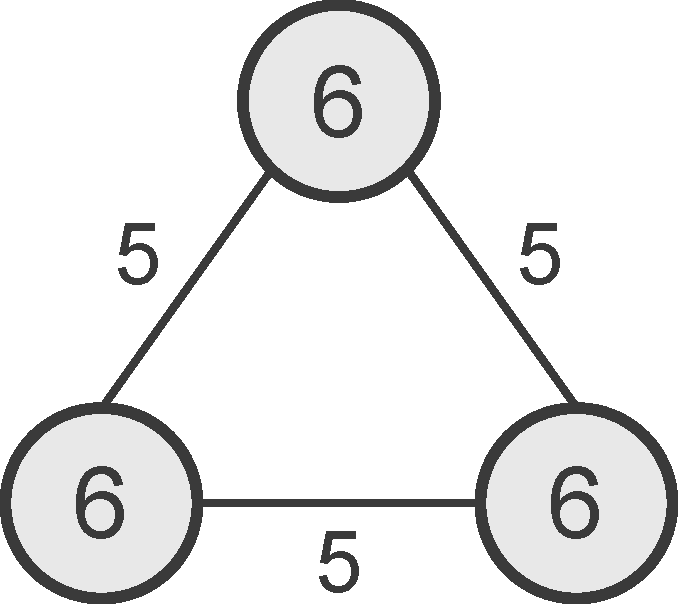
\includegraphics[width=\textwidth]{figures/fig1_vn.pdf}
        \caption{Virtual Network}
        \label{fig:vn}
    \end{subfigure}
    \hfill
    \begin{subfigure}[b]{0.25\textwidth}
        \centering
        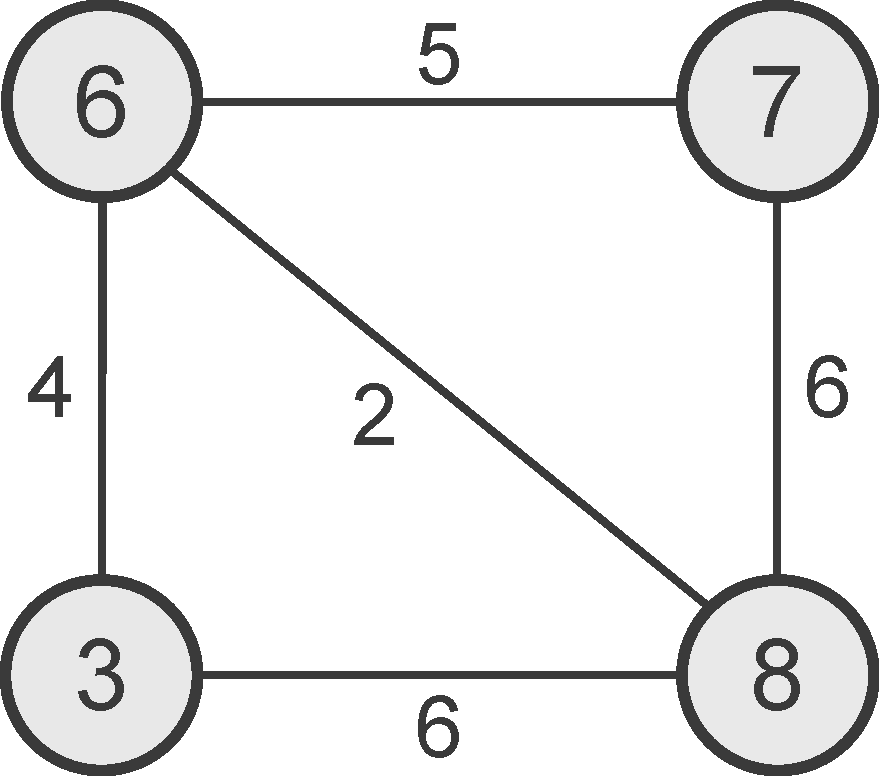
\includegraphics[width=\textwidth]{figures/fig1_sn.pdf}
        \caption{Substrate Network}
        \label{fig:sn}
    \end{subfigure}

    \caption{Example of resource fragmentation in VNE.}
    \label{fig:combined_figures}
\end{figure}

Fig.~\ref{fig:combined_figures} illustrates the resource fragmentation problem. Fig.~\ref{fig:vn}
shows a newly arriving VNR, while Fig.~\ref{fig:sn} represents the residual-resource state of the
substrate network. In terms of aggregate resource capacity, the substrate network may contain
sufficient residual resources to accommodate the request. Nevertheless, the VNR can still be
rejected when these resources cannot be effectively combined to simultaneously satisfy its node and
link requirements.

Thus, the value of a residual resource in VNE is not determined solely by the absolute amount of
remaining CPU or bandwidth. Because a VNR has a graph structure in which nodes and links must be
embedded together, a substrate resource with sufficient residual capacity may still have limited
practical usability if it cannot be effectively combined with surrounding resources for a future
embedding. Resource fragmentation should therefore be evaluated by considering both the amount of
residual resources and their usability. In this work, we represent this usability through external
connectivity and define the External-Connectivity-based Fragmentation (\ecf{}) metric by combining
external connectivity with the residual resource amount.

Node embedding and virtual-link routing require different forms of resource combination. The
residual CPU of a substrate node must be connected to other resources through the bandwidth of its
incident substrate links. In contrast, the residual bandwidth of a substrate link must be
continuously connected with other links so that it can form a substrate path or a larger embedding
structure. We therefore specialize the same external-connectivity principle to substrate nodes and
links according to their respective roles in VNE.

In addition, a change in the fragmentation score before and after an embedding contains two
different effects: direct resource consumption and the degradation in the connectivity of the
resources that remain. These effects should be distinguished. For example, fragmentation may
decrease simply because an already isolated resource is consumed, whereas an appropriate embedding
may instead preserve the connectivity of the remaining resources and prevent further fragmentation.
We therefore separate these two effects and define only the loss caused by the connectivity
degradation of the remaining resources as the \emph{induced fragmentation cost}.

Building on this cost, we formulate the online embedding problem with the induced fragmentation
cost as its objective and propose \ecfvne{}, a greedy embedding algorithm that processes the virtual
nodes of an arriving VNR in breadth-first order and, for each virtual node, evaluates every
CPU-feasible substrate node together with the minimum-hop routing of its pending virtual links.
Every tentative embedding is scored by the induced fragmentation cost relative to the substrate
state observed immediately before the request, so that candidates considered at different stages
of the same VNR are compared on a common basis. Because the external connectivity of a node or a
link is evaluated from the residual bandwidth of its adjacent links alone, the cost of
fragmentation awareness over a plain greedy embedding is small, and the algorithm runs in the order
of milliseconds per request.

The main contributions of this paper are summarized as follows. First, we characterize resource
fragmentation based on the combinability of residual resources rather than solely on their absolute
remaining capacity, and formulate a unified external-connectivity-based \ecf{} metric specialized
for substrate nodes and links. The external connectivity term is defined directly by the residual
capacity of the boundary cut between a resource and its exterior and is monotone under embedding,
which distinguishes it from hop-bounded neighborhood aggregates that depend on tuning parameters. Second, we separate induced fragmentation from the direct effect of resource
consumption, define the non-negative induced fragmentation cost, and incorporate it into an online
node and path selection algorithm, \ecfvne{}, that considers both the current embedding and the
usability of the substrate resources left for future requests. Third, we evaluate \ecfvne{} against
fragmentation-aware and load-balancing-based baselines on a real ISP topology and on FatTree and
BCube data center topologies under a range of arrival rates. Since \ecfvne{} shares its
algorithmic structure with the RFD-based baselines, the comparison primarily reflects the
difference between the fragmentation metrics. The results show that \ecfvne{}
consistently achieves the highest acceptance ratio, revenue, and node utilization, that it
retains this advantage on data center topologies where the existing fragmentation-aware baselines
fall below the load-balancing baselines, and that its margin persists or widens as the offered
load increases.

The remainder of this paper is organized as follows. Section~\ref{sec:related_work} reviews related
work. Section~\ref{sec:system_model} presents the system model, and
Section~\ref{sec:metric_definition_of_resource_fragmentation} defines the \ecf{} metric and the
induced fragmentation cost. Section~\ref{sec:problem_formulation} formulates the embedding problem,
and Section~\ref{sec:embedding_algorithm} describes the \ecfvne{} algorithm and analyzes its
complexity. Section~\ref{sec:performance_evaluation} reports the evaluation results, and
Section~\ref{sec:conclusion} concludes the paper.

\section{Related Work}
\label{sec:related_work}

\subsection{Resource- and Topology-Aware VNE}

Conventional VNE heuristics commonly prioritize candidate substrate nodes according to residual CPU,
residual bandwidth, node degree, centrality, or combinations of these quantities. PageRank-inspired
and other resource-aware node-ranking heuristics use resource and topology information to estimate
the suitability of substrate nodes, followed by virtual link routing through shortest paths or $k$
shortest paths~\cite{cao2017novel,hashmi2020vne}. Other studies use betweenness centrality,
closeness centrality, degree, strength, and multiple topology attributes to guide node
embedding~\cite{ding2015virtual,guler2016closeness,feng2014topology}. More recent multi-criteria
methods further combine several node attributes into a single ranking score. NORD combines
entropy-based weighting with TOPSIS to rank substrate nodes~\cite{tg2023nord}, while simplified
ELECTRE evaluates candidate substrate nodes using multiple node metrics and
constraints~\cite{zhang2018virtual}. These approaches primarily use resource and topology
information to estimate candidate-node suitability for the current embedding decision rather than to
characterize fragmentation of the residual substrate state. The node metric proposed in this paper
also combines residual CPU with adjacent-link bandwidth, but it uses the residual-to-initial ratio
of the adjacent links rather than their absolute amount, and it is applied to the change that an
embedding induces over the whole substrate rather than as a ranking score of the candidate node.

Another line of work coordinates node embedding and link routing because independently selected node
embeddings can lead to infeasible or costly link routings. Coordinated approaches therefore solve
the two mapping operations jointly or through coupled
stages~\cite{chowdhury2012vineyard,lu2023performance,nguyen2022toward}. Related methods extend this
consideration by incorporating congestion, energy consumption, latency, or path characteristics into
embedding decisions~\cite{pham2019congestion,zheng2017link,yan2019latency}. Such coordination
determines how node and link allocation decisions interact and can improve the feasibility or cost
of an embedding. However, coordination and resource fragmentation address different aspects of VNE:
coordination determines how an embedding is constructed, whereas fragmentation metrics characterize
the usability of the residual resources left by that embedding.

Load-balancing approaches address another related aspect by discouraging excessive resource
concentration on particular substrate nodes or
links~\cite{gong2014toward,shanbhag2015vhub,li2022load}. Some load-balancing methods additionally
use global resource information or neighboring bandwidth when evaluating node-embedding potential.
These objectives seek a balanced distribution of substrate utilization. Resource balance and
resource fragmentation, however, are not equivalent. From the fragmentation perspective adopted in
this paper, the relevant question is whether a residual resource can still be used together with the
other resources required by a future mapping operation, rather than only whether residual resources
are evenly distributed across the substrate network. Load balancing is therefore not part of the
proposed objective; representative load-balancing algorithms are instead used as baselines in
Section~\ref{sec:performance_evaluation}.

% \subsection{Survivable VNE Under Substrate Failures}

% Survivable VNE addresses service availability under substrate failures. Prior studies reserve backup
% paths or redundant node and link resources, construct backup topologies, or remap affected virtual
% components after
% failures~\cite{liao2014survivable,chowdhury2016dedicated,liu2017scheme,zheng2019heuristic,sun2011framework,zhu2014heuristic}.
% Shahriar et al.~\cite{shahriar2019virtual} formulate Connectivity-aware Virtual Network Embedding
% (CoViNE), which guarantees VN connectivity under multiple substrate link failures without requiring
% full bandwidth protection. CoViNE uses VN augmentation and disjointness requirements to preserve
% connectivity after failures. Survivable VNE concerns whether an embedded VN can continue to satisfy
% a survivability requirement after substrate failures, whereas this paper considers the usability of
% residual resources resulting from online embedding decisions under normal operation.

\subsection{Fragmentation-Aware VNE}

The following studies are most closely related to the fragmentation notion considered in this paper.
Fragmentation-aware VNE explicitly considers residual resources that become difficult to use despite
remaining available.

Guan et al.~\cite{guan2023multidimensional} study multidimensional resource fragmentation for VNE in
MEC systems interconnected by optical networks. For physical nodes, their formulation characterizes
fragmentation through imbalanced utilization of computing and wireless resources. For physical
links, it identifies unusable or difficult-to-use optical spectrum fragments created under spectrum
continuity and consistency constraints. Their bilevel formulation also accounts for the dependency
between virtual node embedding and virtual link routing. Thus, their fragmentation model focuses on
imbalance among heterogeneous node resources and contiguity of optical spectrum resources, which
differs from the CPU--bandwidth resource relationships addressed in this paper. Whereas this paper
treats node and link fragmentation as two instances of the same general form $F=R(1-\mathrm{Conn})$,
Guan et al. formulate two problems with different characteristics: node imbalance and link spectrum
continuity.

Lu and Zhang~\cite{lu2022resource} address a more closely related notion of resource fragmentation.
They define the resource fragmentation degree (RFD) for substrate nodes and links based on the
observation that the usability of a residual resource depends on surrounding residual resources. For
a substrate node, RFD incorporates residual resources of neighboring nodes and paths within a
bounded hop count. For a substrate link, RFD incorporates the residual resources of adjacent links
and the substrate nodes shared by those links. Their formulation is motivated by an extension of
graph connectivity and aggregates these surrounding resource states to quantify the fragmentation
degree of each substrate element. This connectivity extension depends on a hop-bounded neighborhood
and its associated hyperparameter, whereas the external connectivity used in this paper is defined
directly by the residual capacity of the boundary cut and requires no hop-count tuning. Their
embedding algorithm, VNE-RFD, processes the virtual nodes of a request sequentially from a root
selected by degree and resource demand, evaluates every CPU-feasible substrate node for each virtual
node, and minimizes the sum of the embedding cost and the residual-weighted fragmentation degree
of the whole substrate after the embedding. The latter is an absolute quantity that decreases
whenever an already fragmented resource is consumed; in contrast, the induced cost proposed in
this paper isolates the connectivity degradation of the resources that remain.

The proposed metric shares with RFD the observation that residual resource amount alone is
insufficient to characterize future usability. The distinction lies in how the relevant resource
relationships are modeled. Rather than deriving a connectivity-inspired fragmentation degree from
surrounding nodes and paths, the proposed metric directly follows the resource combinations required
by the two VNE mapping operations. For node embedding, it evaluates the residual resource of a
substrate node together with the residual resources of its adjacent substrate links, because both
are required to support a virtual node and its incident virtual links. For link routing, it
evaluates the residual resource of a substrate link together with the adjacent link resources at
each of its two endpoints. The two endpoint states are evaluated separately, and the endpoint with
lower adjacent-resource availability determines the resulting value because insufficient adjacent
resources at either endpoint can limit the use of the substrate link as part of a path.

Accordingly, the proposed metric differs from the reviewed fragmentation metrics not in whether
neighboring resources are considered, but in how their relationships are defined. It characterizes
residual-resource usability according to the distinct resource combinations required by node
embedding and link routing, aiming to identify residual resources that remain available but are
difficult to combine with other resources in future VNR embeddings. In addition, the formulation
distinguishes the direct resource-consumption effect of an embedding from the connectivity
degradation it induces, with the latter represented through the external connectivity metric
introduced in the next section.

\begin{table}[!t]
\caption{\textbf{Notation specification}}
\label{tab:notation}
\centering
\setlength{\tabcolsep}{3pt}
\renewcommand{\arraystretch}{1.12}

\begin{tabular}{|p{0.30\columnwidth}|p{0.60\columnwidth}|}
\hline
\textbf{Symbol} & \textbf{Description} \\
\hline

$G^S=(N^S,L^S)$
& Substrate network \\
\hline

$G^V=(N^V,L^V)$
& Virtual network request \\
\hline

$c_v,\;r_v$
& Initial and residual CPU capacities of substrate node $v$ \\
\hline

$c_e,\;r_e$
& Initial and residual bandwidth capacities of substrate link $e$ \\
\hline

$\mathrm{Conn}_N,\;\mathrm{Conn}_L$
& External-connectivity measures for substrate nodes and links \\
\hline

$I_N,\;I_L$
& Connectivity-deficiency factors for substrate nodes and links \\
\hline

$\Delta F_N,\;\Delta F_L$
& Induced node and link fragmentation \\
\hline

$J_{\mathrm{ECF}}$
& Induced fragmentation cost (embedding objective) \\
\hline

$\beta,\;\gamma$
& Weights of link and node fragmentation terms \\
\hline

\end{tabular}
\end{table}

\section{System Model}
\label{sec:system_model}

We model the substrate network as a weighted undirected graph $G^S=(N^S,L^S)$, where $N^S$ and $L^S$
denote the sets of substrate nodes and substrate links, respectively; the main notation used
throughout the paper is summarized in Table~\ref{tab:notation}. For each substrate node $v\in
N^S$, we let $c_v$ and $r_v$ denote its initial and current residual CPU capacities, and for each
substrate link $e=\{u,v\}\in L^S$, we let $c_e$ and $r_e$ denote its initial and current residual
bandwidth capacities. To represent paths and flows for virtual-link routing, we expand each
undirected substrate link $\{u,v\}\in L^S$ into two directed arcs $(u,v)$ and $(v,u)$, and we
collect these arcs into the set $A^S$.

We represent a VNR as a weighted undirected graph $G^V=(N^V,L^V)$. Here $N^V$ and $L^V$ are the sets
of virtual nodes and virtual links, respectively; we let $d_n$ denote the CPU demand of virtual node
$n\in N^V$, and $d_l$ the bandwidth demand of virtual link $l=\{n,m\}\in L^V$.

We define the node mapping as $M_N:N^V\rightarrow N^S$. Each virtual node is mapped to exactly one
substrate node, and we assume that distinct virtual nodes of the same VNR are mapped to distinct
substrate nodes. We use the binary variable $x_{nv}\in\{0,1\}$, where $x_{nv}=1$ indicates that
virtual node $n$ is mapped to substrate node $v$. We define the link mapping as
$M_L:L^V\rightarrow\mathcal{P}^S$, where each virtual link $l=\{n,m\}$ is mapped to substrate paths
connecting $M_N(n)$ and $M_N(m)$. We let $f_{uv}^l\ge0$ denote the bandwidth flow of virtual link
$l$ that traverses arc $(u,v)\in A^S$.

We define the complete VNR embedding as $M=(M_N,M_L)$. After applying an embedding $M$, we update
the residual resources of substrate nodes and substrate links, respectively, as
\begin{equation}
    r_v(M)
    =
    r_v-\sum_{n\in N^V}d_nx_{nv},
    \qquad \forall v\in N^S,
\label{eq:res_node}
\end{equation}
\begin{equation}
    r_{\{u,v\}}(M)
    =
    r_{\{u,v\}}
    -
    \sum_{l\in L^V}
    \left(
    f_{uv}^l+f_{vu}^l
    \right),
    \qquad
    \forall\{u,v\}\in L^S.
\label{eq:res_link}
\end{equation}
The pre- and post-embedding residual substrate states given by \eqref{eq:res_node} and
\eqref{eq:res_link} serve as the basis for computing
the \ecf{} metric and the induced fragmentation cost in the following sections.

\section{External-Connectivity-Based Fragmentation Metric}
\label{sec:metric_definition_of_resource_fragmentation}

We now define the External-Connectivity-based Fragmentation (\ecf) metric, which combines residual
amount and external connectivity to represent the future usability of a residual resource. The
\ecf{} metric uses a common base form for nodes and links, but specializes to reflect the different
ways in which each resource combines with other resources in VNE.

\subsection{Base Definition and External Connectivity}
In VNE, the usability of a residual resource depends not only on its amount but also on its
combinability with surrounding resources. Let $R$ denote the residual amount and $\mathrm{Conn}$ the
normalized external connectivity; we view $R\cdot\mathrm{Conn}$ as the effectively usable portion of
the residual resource that can combine with external resources. We accordingly define the
fragmentation score as
\begin{equation}
    F=R(1-\mathrm{Conn}).
\label{eq:base_frag}
\end{equation}
When $\mathrm{Conn}$ approaches one, the residual resource can be combined with external resources
sufficiently and fragmentation is small; in contrast, as external connectivity decreases, the
fragmentation score grows for the same residual amount.

To make external connectivity concrete, we consider any $\emptyset\neq A\subsetneq N^S$ and let
$\bar A=N^S\setminus A$. We define the boundary link set that connects the region $A$ with its
exterior $\bar A$ as
\begin{equation}
    \delta(A)
    =
    \{\,e=\{u,v\}\in L^S
    \mid
    u\in A,\ v\in\bar A\,\}.
\label{eq:boundary}
\end{equation}
The initial and residual bandwidth capacities of this boundary are given, respectively, by
$\sum_{e\in\delta(A)}c_e$ and $\sum_{e\in\delta(A)}r_e$, and we define the normalized external
connectivity as
\begin{equation}
    \mathrm{Conn}(A)
    =
    \begin{cases}
        \dfrac{\sum_{e\in\delta(A)}r_e}{\sum_{e\in\delta(A)}c_e},
         & \sum_{e\in\delta(A)}c_e>0, \\[1mm]
        0,
         & \sum_{e\in\delta(A)}c_e=0.
    \end{cases}
\label{eq:conn}
\end{equation}
Since any bandwidth exchanged between $A$ and $\bar A$ must traverse $\delta(A)$, the residual
capacity of this boundary is the total bandwidth available for region $A$ to connect with its
exterior, and $\mathrm{Conn}(A)$ expresses it as a fraction of the initial boundary capacity.

Two properties motivate this choice of connectivity term. First, $\mathrm{Conn}(A)$ bounds the
external usability of $A$: if $\mathrm{Conn}(A)=0$, no additional bandwidth can cross the boundary,
and the resources inside $A$ cannot be combined with any external resource regardless of how a
demand is routed. Second, $\mathrm{Conn}$ is monotone under embedding: because every
embedding only removes bandwidth from $\delta(A)$, we have
$\sum_{e\in\delta(A)}r_e(M)\le\sum_{e\in\delta(A)}r_e$ and therefore
\begin{equation}
    \mathrm{Conn}(A;M)\le\mathrm{Conn}(A),
    \qquad
    \forall\,\emptyset\neq A\subsetneq N^S,
\label{eq:monotone}
\end{equation}
where $\mathrm{Conn}(A;M)$ denotes the external connectivity evaluated in the residual state after
embedding $M$. These two properties keep the metric
interpretable as a resource-usability bound whose external connectivity cannot improve merely as a
byproduct of embedding.

In the remainder of this section, the region $A$ is instantiated as a single substrate node or as
the endpoints of a single substrate link, which are the smallest resource combinations required by
node embedding and virtual-link routing, respectively. This choice keeps the evaluation of
$\mathrm{Conn}$ local to the adjacent links of a resource; the definition itself applies to larger
regions without modification. Normalizing by the initial boundary capacity makes $\mathrm{Conn}$
independent of the absolute bandwidth scale, so that node and link fragmentation can be expressed
in a common form and combined across resource types.

\subsection{Node Fragmentation}
For a substrate node $v\in N^S$, we set $A=\{v\}$ in \eqref{eq:conn}, so that the external
connectivity of the node is given by
\begin{equation}
    \mathrm{Conn}_N(v)
    =
    \begin{cases}
        \dfrac{\sum_{e\in\delta(\{v\})}r_e}
        {\sum_{e\in\delta(\{v\})}c_e},
         & \sum_{e\in\delta(\{v\})}c_e>0, \\[1mm]
        0,
         & \text{otherwise.}
    \end{cases}
\label{eq:conn_n}
\end{equation}
In VNE, the residual CPU of a substrate node must combine with the bandwidth of its adjacent links
to reach other substrate resources; therefore, a reduction in adjacent bandwidth lowers the future
usability of that CPU. Accordingly, we define the node connectivity-deficiency factor and the node
fragmentation score as
\begin{equation}
    I_N(v)=1-\mathrm{Conn}_N(v),
    \qquad
    F_N(v)=r_v I_N(v).
\label{eq:node_frag}
\end{equation}

\subsection{Link Fragmentation}

For a substrate link $e=\{u,v\}\in L^S$, its residual bandwidth is useful
for future virtual-link embeddings only when the link can be extended
through residual bandwidth resources around its endpoints. We therefore
evaluate the external connectivity of $e$ separately at $u$ and $v$, while
excluding $e$ itself from the neighboring-link set of each endpoint.

For an endpoint $z\in\{u,v\}$, the set of external substrate links incident to $z$, excluding $e$
itself, is $\delta(\{z\})\setminus\{e\}$. Whenever the total initial capacity of these links is
positive, the endpoint connectivity of $z$ with respect to $e$ is defined as their
residual-to-initial capacity ratio,
\begin{equation}
    \mathrm{Conn}_z(e)
    =
    \frac{\sum_{e'\in\delta(\{z\})\setminus\{e\}}r_{e'}}
         {\sum_{e'\in\delta(\{z\})\setminus\{e\}}c_{e'}},
    \qquad
    \sum_{e'\in\delta(\{z\})\setminus\{e\}}c_{e'}>0.
\label{eq:conn_endpoint}
\end{equation}
If that total initial capacity is zero, endpoint $z$ has no external link resource through which
$e$ can be extended; this endpoint is excluded from the link-connectivity comparison rather than
assigned an artificial connectivity value.

The external connectivity of $e$ is determined by the minimum endpoint connectivity among the endpoints that possess external link resources, defined as $\mathcal{Z}_e = \left\{ z \in \{u, v\} \;\middle|\; \sum_{e' \in \delta(z) \setminus \{e\}} c_{e'} > 0 \right\}$:
\begin{equation}
\mathrm{Conn}_L(e) = 
\begin{cases}
    \displaystyle \min_{z \in \mathcal{Z}_e} \mathrm{Conn}_z(e), & \text{if } \mathcal{Z}_e \neq \emptyset, \\[1.5ex]
    0, & \text{otherwise.}
\end{cases}
\label{eq:conn_l}
\end{equation}
Accordingly, three cases arise naturally. If both endpoints have external link resources, the
smaller of their two connectivity values is used. If only one endpoint has external link
resources, the connectivity of that endpoint is used. If neither endpoint has an external link
resource, the link has no external extension opportunity, and its external connectivity is zero.

The link connectivity-deficiency factor and link fragmentation score are then given by
\begin{equation}
    I_L(e)=1-\mathrm{Conn}_L(e),
    \qquad
    F_L(e)=r_e I_L(e).
\label{eq:link_frag}
\end{equation}

This definition applies a bottleneck principle only when a comparison is
meaningful. It does not penalize a link merely because one endpoint is a
leaf-like endpoint with no other incident substrate link. However, when
both endpoints lack external neighboring resources, the residual bandwidth
of the link is fully isolated; hence $\mathrm{Conn}_L(e)=0$ and
$I_L(e)=1$.

\subsection{Induced Fragmentation Cost}

The difference between the pre- and post-embedding fragmentation scores
contains both the direct effect of resource consumption and the effect of
connectivity degradation on the resources that remain. For a general
fragmentation score $F=RI$, the change caused by an embedding $M$ can be
decomposed as
\begin{equation}
F(M)-F
=
\bigl(R(M)-R\bigr)I
+
R(M)\bigl(I(M)-I\bigr).
\label{eq:decomp}
\end{equation}
The first term represents the direct consumption of the resource itself.
The second term represents the additional loss of usability caused by the
degraded connectivity of the residual resource after embedding. Since the
purpose of the proposed metric is to quantify fragmentation of the
resources that remain available for future VNRs, we retain only the second
term.

For each arriving VNR, let $S_0$ denote the residual substrate state
immediately before the VNR is processed, and let $S(M)$ denote the residual
state after applying a partial or complete embedding $M$. Applying the second term of
\eqref{eq:decomp} to every substrate node and link, the induced node fragmentation and the induced
link fragmentation are defined as
\begin{equation}
\begin{aligned}
\Delta F_N(M)
=
\sum_{v\in N^S}
r_v(S(M))
\left(
I_N(v;S(M))-I_N(v;S_0)
\right),
\label{eq:delta_fn}
\end{aligned}
\end{equation}

\begin{equation}
\Delta F_L(M)
=
\sum_{e\in L^S}
r_e(S(M))
\left(
I_L(e;S(M))-I_L(e;S_0)
\right),
\label{eq:delta_fl}
\end{equation}
where $I_N(\cdot;S)$ and $I_L(\cdot;S)$ denote the connectivity-deficiency factors
\eqref{eq:node_frag} and \eqref{eq:link_frag} evaluated in state $S$.

Both quantities are non-negative by construction. Because an embedding only consumes substrate
resources and removes bandwidth from the associated boundary, the monotonicity property
\eqref{eq:monotone} implies that the external connectivity of a node or link cannot increase, i.e.,
$I_N(v;S(M))-I_N(v;S_0)\ge0$ for every $v\in N^S$ and $I_L(e;S(M))-I_L(e;S_0)\ge0$ for every $e\in
L^S$; the residual-resource factors $r_v(S(M))$ and $r_e(S(M))$ are non-negative for any feasible
embedding. The residual-resource factors ensure that \eqref{eq:delta_fn} and \eqref{eq:delta_fl}
penalize degradation in the usability of resources that remain available after the embedding,
rather than merely charging the resources that have already been consumed. In terms of embedding
decisions, $\Delta F_N$ penalizes bandwidth consumption on links adjacent to nodes with large
residual CPU, and $\Delta F_L$ penalizes bandwidth consumption adjacent to links with large
residual bandwidth; an embedding with low induced cost therefore consumes bandwidth near
resources that are already utilized and leaves well-connected residual resources intact.

\section{Problem Formulation}
\label{sec:problem_formulation}

The objective of \ecfvne{} is to embed the current VNR while preserving the
future usability of residual substrate resources. For each arriving VNR, let
$S_0$ denote the residual substrate state immediately before the request is
processed, and let $S(M)$ denote the residual state after a partial or
complete embedding $M$; the reference state $S_0$ remains fixed throughout
processing of the current request. The decision variable
$x_{nv}\in\{0,1\}$ indicates whether virtual node $n\in N^V$ is mapped to
substrate node $v\in N^S$, and $f_{uv}^l\ge0$ denotes the bandwidth of
virtual link $l$ routed through substrate arc $(u,v)\in A^S$.

\textbf{Objective:}

\ecfvne{} ranks feasible tentative embeddings $M$ of the current VNR by the
induced fragmentation cost they impose on the substrate network:
\begin{equation}
\text{minimize}\quad
J_{\mathrm{ECF}}(M)
=
\beta\,\Delta F_L(M)
+
\gamma\,\Delta F_N(M),
\qquad
\beta,\gamma\ge0,
\label{eq:objective}
\end{equation}
where $\Delta F_L(M)$ and $\Delta F_N(M)$ are the induced link and node fragmentation defined in
\eqref{eq:delta_fl} and \eqref{eq:delta_fn}, both evaluated relative to the fixed reference state
$S_0$, and $\beta$ and $\gamma$ control the contributions of link and node fragmentation,
respectively.

\textbf{Constraints:}

\textbf{--- Node Assignment Constraints:}
\begin{equation}
\sum_{v\in N^S}x_{nv}=1,
\qquad
\forall n\in N^V,
\label{eq:node_assign}
\end{equation}
\begin{equation}
\sum_{n\in N^V}x_{nv}\le1,
\qquad
\forall v\in N^S.
\label{eq:node_unique}
\end{equation}

\textbf{--- Capacity Constraints:}
\begin{equation}
\sum_{n\in N^V}d_nx_{nv}
\le r_v,
\qquad
\forall v\in N^S,
\label{eq:cpu_cap}
\end{equation}
\begin{equation}
\sum_{l\in L^V}
\left(
 f_{uv}^l+f_{vu}^l
\right)
\le r_{\{u,v\}},
\qquad
\forall\{u,v\}\in L^S.
\label{eq:bw_cap}
\end{equation}

\textbf{--- Flow Conservation Constraints:}
\begin{equation}
\begin{aligned}
\sum_{(v,w)\in A^S}f_{vw}^l
-
\sum_{(w,v)\in A^S}f_{wv}^l
&=
 d_l\left(x_{nv}-x_{mv}\right),
\\
&\forall v\in N^S,\quad
\forall l=\{n,m\}\in L^V.
\end{aligned}
\label{eq:flow_cons}
\end{equation}

\textbf{Remarks:}
\begin{itemize}
    \item The objective~\eqref{eq:objective} is non-negative, since both \eqref{eq:delta_fl} and
    \eqref{eq:delta_fn} are non-negative by the monotonicity property~\eqref{eq:monotone}. The two
    terms are not normalized by substrate-wide resource capacities; therefore, the weights $\beta$
    and $\gamma$ also account for possible differences in the numerical scales of CPU and bandwidth
    resources.
    \item Constraint sets~\eqref{eq:node_assign} and~\eqref{eq:node_unique} enforce that each virtual
    node is mapped to exactly one substrate node and that distinct virtual nodes of the same VNR are
    not mapped to the same substrate node.
    \item Constraint~\eqref{eq:cpu_cap} ensures that the CPU demand allocated to a substrate node
    does not exceed its current residual CPU capacity.
    \item Constraint~\eqref{eq:bw_cap} ensures that the total bandwidth allocated on an undirected
    substrate link, summed over both directions, does not exceed its residual bandwidth.
    \item Constraint~\eqref{eq:flow_cons} enforces flow conservation for each virtual link
    $l=\{n,m\}\in L^V$: the net flow at every substrate node is zero, except at the substrate nodes
    hosting $n$ and $m$, which act as the source and destination of $l$'s routed flow.
\end{itemize}

\section{\ecfvne{} Embedding Algorithm}
\label{sec:embedding_algorithm}

\begin{algorithm}[!t]
\caption{\ecfvne{} Main Greedy Embedding Algorithm}
\label{alg:ecf_main}
\footnotesize
\begin{algorithmic}[1]
\STATE \textbf{Input:} substrate network $G^S$, VNR $G^V$, weights
$\beta$ and $\gamma$
\STATE \textbf{Output:} embedding $M$ or rejection
\STATE $S_0\leftarrow$ current residual state of $G^S$
\STATE Select root $r\in N^V$ by lexicographically maximizing
$\left(\deg(n),d_n,\sum_{l\in L^V:n\in l}d_l\right)$
\STATE Obtain BFS processing order $\pi$ from $r$
\STATE $M\leftarrow\emptyset$
\STATE $v_r\leftarrow$\textsc{RootPlacement}$(G^S,r)$
\IF{$v_r=\emptyset$}
    \STATE \textbf{return} CPU rejection
\ENDIF
\STATE $M\leftarrow M\cup\{r\mapsto v_r\}$

\FOR{each virtual node $n\in\pi\setminus\{r\}$}
    \STATE $\mathcal{C}\leftarrow\emptyset$
    \STATE $\mathit{hasCpuCandidate}\leftarrow\textbf{false}$

    \FOR{each substrate node $v\in N^S$}
        \IF{$v$ is used by $M_N$ \OR $r_v<d_n$}
            \STATE \textbf{continue}
        \ENDIF

        \STATE $\mathit{hasCpuCandidate}\leftarrow\textbf{true}$
        \STATE $\widehat{M}\leftarrow M\cup\{n\mapsto v\}$
        \STATE $\mathit{feasible}\leftarrow\textbf{true}$
        \STATE $\mathcal{L}_n\leftarrow
        \{l=\{n,m\}\in L^V:m\text{ is mapped in }M\}$

        \FOR{each $l=\{n,m\}\in\mathcal{L}_n$ in increasing link-index order}
            \STATE $p\leftarrow$\textsc{MinimumHopPath}
            $(G^S,v,M_N(m),d_l)$
            \IF{$p=\emptyset$}
                \STATE $\mathit{feasible}\leftarrow\textbf{false}$
                \STATE \textbf{break}
            \ENDIF
            \STATE $\widehat{M}\leftarrow\widehat{M}\cup\{l\mapsto p\}$
        \ENDFOR

        \IF{$\mathit{feasible}$}
            \STATE $\mathcal{C}\leftarrow\mathcal{C}\cup
            \{(\widehat{M},J_{\mathrm{ECF}}(\widehat{M}))\}$
        \ENDIF
    \ENDFOR

    \IF{$\mathcal{C}=\emptyset$}
        \IF{\textbf{not} $\mathit{hasCpuCandidate}$}
            \STATE \textbf{return} CPU rejection
        \ELSE
            \STATE \textbf{return} routing rejection
        \ENDIF
    \ENDIF

    \STATE $(M,\cdot)\leftarrow
    \arg\min_{(\widehat{M},J)\in\mathcal{C}} J$
\ENDFOR
\STATE \textbf{return} $M$
\end{algorithmic}
\end{algorithm}


\begin{algorithm}[!t]
\caption{RootPlacement}
\label{alg:root_placement}
\footnotesize
\begin{algorithmic}[1]
\STATE \textbf{Input:} substrate network $G^S$, root virtual node $r$
\STATE \textbf{Output:} substrate node $v_r$ or $\emptyset$
\STATE $v_r\leftarrow\emptyset$
\STATE $I^*\leftarrow+\infty$
\STATE $R^*\leftarrow-1$

\FOR{each substrate node $v\in N^S$}
    \IF{$r_v<d_r$}
        \STATE \textbf{continue}
    \ENDIF

    \STATE $I\leftarrow I_N(v)$
    \IF{$v_r=\emptyset$ \OR $I<I^*$
    \OR $(I=I^* \AND r_v>R^*)$
    \OR $(I=I^* \AND r_v=R^* \AND v<v_r)$}
        \STATE $v_r\leftarrow v$
        \STATE $I^*\leftarrow I$
        \STATE $R^*\leftarrow r_v$
    \ENDIF
\ENDFOR

\STATE \textbf{return} $v_r$
\end{algorithmic}
\end{algorithm}

This section presents the \ecfvne{} algorithm, summarized in Algorithm~\ref{alg:ecf_main}, for
sequentially embedding an arriving VNR. Let $S_0$ denote the residual substrate state immediately
before the VNR is processed. The algorithm preserves $S_0$ as a fixed
reference state and evaluates every feasible partial embedding $M$ using
the objective $J_{\mathrm{ECF}}(M)$ defined in
\eqref{eq:objective}. Therefore, candidates considered at
different stages of the same VNR are compared according to the cumulative
fragmentation that they induce relative to the same pre-request substrate
state. Unless noted otherwise, whenever a selection rule below leaves multiple candidates
lexicographically or numerically tied, the tie is broken deterministically by the smaller index
of the corresponding virtual or substrate entity.

The algorithm begins by selecting a root virtual node, namely the one that lexicographically
maximizes the tuple $\bigl(\deg(n),\,d_n,\,\sum_{l\in L^V:n\in l}d_l\bigr)$. This choice
prioritizes virtual nodes that have more incident constraints and larger resource requirements.
Starting from the selected root, the remaining virtual nodes are processed in breadth-first
order. If the VNR contains more than one connected component, the traversal resumes from the
smallest-index unvisited virtual node after completing each component.

The root substrate node is selected by \textsc{RootPlacement} (Algorithm~\ref{alg:root_placement}),
namely the substrate node with
enough residual CPU for the root demand that lexicographically minimizes node isolation and
maximizes residual CPU capacity, i.e., it chooses the node with the minimum node isolation,
breaking ties by the larger residual CPU capacity. This rule favors a resource-rich substrate
location whose neighboring bandwidth remains comparatively well connected.

After root placement, \ecfvne{} processes each remaining virtual node $n$.
It considers every substrate node $v$ that has sufficient residual CPU and
has not already been assigned to another virtual node of the same VNR. For
each such candidate, the algorithm makes a temporary copy of the current
partial embedding, maps $n$ to $v$, and identifies the virtual links from
$n$ to already mapped virtual neighbors. Those pending virtual links are
processed in increasing virtual-link index order.

For a pending virtual link $l=\{n,m\}$, the algorithm uses breadth-first
search to find a single minimum-hop path from $v$ to $M_N(m)$. During the
search, a substrate link is traversable only if its current residual
bandwidth satisfies the demand of $l$. When several minimum-hop paths are
available, the search resolves the choice by the index-based tie-breaking rule stated above.
The demand of $l$ is allocated immediately after the path is found, so the
routing decision for a later pending link reflects the resource consumption
of earlier links in the same tentative candidate.

A candidate substrate node is infeasible if any pending virtual link cannot
be routed. Otherwise, its resulting tentative embedding is evaluated by
$J_{\mathrm{ECF}}$, which measures the induced node and link fragmentation
relative to $S_0$. Among all feasible candidates, the algorithm commits the
one with the minimum objective value. The algorithm is greedy: after a candidate is
committed, earlier node and link decisions are not revisited. A VNR is
rejected due to CPU infeasibility when no unused substrate node can satisfy
the current virtual-node CPU demand. It is rejected due to routing
infeasibility when CPU-feasible candidates exist but none can route all of
their required pending virtual links.

\subsection{Complexity Analysis}

Let $\Delta_S$ denote the maximum degree of a substrate node. Because the algorithm maps distinct
virtual nodes of the same VNR to distinct substrate nodes, a feasible request always satisfies
$|N^V|\le|N^S|$.

For each virtual node, \ecfvne{} examines at most $|N^S|$ substrate-node candidates, so the aggregate
candidate-enumeration cost is $O(|N^S||N^V|)$. Each virtual link is routed exactly once, when its
second endpoint is mapped. For each tested substrate-node candidate, routing a pending virtual link
requires a bandwidth-feasible minimum-hop breadth-first search, which costs $O(|N^S|+|L^S|)$;
therefore, the aggregate path-search cost is $O\bigl(|N^S||L^V|(|N^S|+|L^S|)\bigr)$.

For one ECF objective evaluation, all node-isolation values can be obtained by scanning substrate
links once, which costs $O(|L^S|)$. For link isolation, the external links incident to both
endpoints of every substrate link are examined, at a total cost of
$O\bigl(\sum_{v\in N^S}\deg(v)^2\bigr)=O(|L^S|\Delta_S)$. Thus, one evaluation of
$J_{\mathrm{ECF}}$ costs $O(|L^S|\Delta_S)$, and since at most $O(|N^S||N^V|)$ candidate embeddings
are evaluated, the total objective-evaluation cost is $O\bigl(|N^S||N^V||L^S|\Delta_S\bigr)$.

The overall worst-case running time is therefore
\begin{equation}
O\Bigl(
|N^S||N^V|
+
|N^S||L^V|\bigl(|N^S|+|L^S|\bigr)
+
|N^S||N^V||L^S|\Delta_S
\Bigr).
\label{eq:complexity}
\end{equation}
This bound depends on both the substrate topology ($|N^S|$, $|L^S|$, $\Delta_S$) and the size of the
arriving VNR ($|N^V|$, $|L^V|$); we keep these request-side quantities explicit rather than
expressing them in terms of the substrate size, since the size of a VNR is independent of the
substrate network. To characterize how substrate topology affects this bound, we consider two
representative regimes. For a sparse substrate, where $|L^S|=O(|N^S|)$ and $\Delta_S=O(1)$, the
running time reduces to $T_{\mathrm{sparse}}=O\bigl(|N^S|^2|N^V|+|N^S|^2|L^V|\bigr)$. For a dense
substrate, where $|L^S|=O(|N^S|^2)$ and $\Delta_S=O(|N^S|)$, it reduces to
$T_{\mathrm{dense}}=O\bigl(|N^S|^4|N^V|+|N^S|^3|L^V|\bigr)$.

\section{Performance Evaluation}
\label{sec:performance_evaluation}

This section evaluates \ecfvne{} against representative fragmentation-aware and load-balancing-based
VNE algorithms on an ISP topology and two data center network (DCN) topologies. We first describe
the simulation setup, the compared algorithms, the network settings, and the performance metrics,
and then present the results under a fixed VNR arrival rate followed by the results under
increasing arrival rates.

\subsection{Evaluation Setup}

All algorithms are implemented and evaluated within the VIRNE simulation
environment~\cite{wang_virne}. We consider a dynamic online VNE scenario in which VNRs arrive
according to a Poisson process and stay in the substrate network for an exponentially distributed
lifetime, after which their resources are released. Each substrate network--algorithm pair is
evaluated over at least 10 independent simulation runs with different random seeds, and the
reported values are averaged over these runs. To capture steady-state behavior, an initial warm-up
period equal to ten times the mean VNR lifetime is excluded from the measurement, and each run is
then measured over 50{,}000 time units.

\subsection{Compared Algorithms}

We compare \ecfvne{} with two groups of baselines. The first group consists of the
resource-fragmentation-based algorithms VNE-RFD-B and VNE-RFD-D~\cite{lu2022resource}, which embed
each VNR so as to minimize the resource fragmentation degree (RFD) reviewed in
Section~\ref{sec:related_work}; the two variants differ only in whether the virtual nodes following
the root are ordered by breadth-first or depth-first search. The
second group consists of the load-balancing-based algorithms D-ViNE and
R-ViNE~\cite{chowdhury2012vineyard}, which coordinate node and link mapping through a relaxed
mixed-integer program and select substrate nodes by deterministic and randomized rounding,
respectively. For VNE-RFD-B and VNE-RFD-D, the backtracking bound, the number of candidate paths,
and the hop bound of the fragmentation neighborhood are set to $\Delta=100$, $K=10$, and $\tau=3$
for computational tractability. Placement-location constraints are disabled for all algorithms so
that every substrate node with sufficient CPU is a valid candidate. Unless otherwise specified, the
remaining algorithm-specific parameters follow the settings reported in the original papers. For
\ecfvne{}, both weighting factors of the objective are set to $\beta=\gamma=1$ without
topology-specific tuning.

VNE-RFD-B shares its overall structure with \ecfvne{}: the root virtual node is selected by degree
and resource demand, the remaining virtual nodes are processed in breadth-first order, and every
CPU-feasible substrate node is evaluated for each virtual node. The two algorithms differ in the
fragmentation metric that drives node selection, in the path search ($K$ candidate paths versus a
single minimum-hop path), in the root placement rule, and in the presence of backtracking, which
\ecfvne{} does not use. The comparison with VNE-RFD-B therefore primarily reflects the difference
between the two fragmentation metrics.

\subsection{Network Settings}

\subsubsection{Substrate Networks}

We use three substrate networks that represent two distinct deployment environments. As an ISP
network, we adopt the Columbus topology from the Internet Topology Zoo~\cite{knight2011internet},
which consists of 70 nodes and 85 links. Its node CPU capacities and link bandwidth capacities are
drawn uniformly from $U[50,100]$ and $U[250,500]$, respectively, so that the substrate is
heterogeneous both in topology and in capacity.

As DCNs, we adopt a FatTree topology (FT6) with 64 hosts and 45 switches and a BCube topology,
BCube$(2,4)$, with 64 hosts and 48 switches. In both DCNs, each host has a CPU capacity of 100 and
every link has a bandwidth capacity of 100. Switches have zero CPU capacity; virtual nodes can be
mapped only onto hosts, and switches are used solely for forwarding virtual links. The two DCNs
therefore share the same number of hosts and the same per-element capacities but differ in how
hosts attach to the fabric: in FT6 each host is connected to the network through a single link,
whereas in BCube$(2,4)$ each host is connected to multiple switches at different levels.

\subsubsection{Virtual Network Requests}

Each VNR has a number of virtual nodes drawn from the discrete uniform distribution over $[2,10]$,
and its topology is a connected Erd\H{o}s--R\'enyi graph with connection probability $p=0.4$.
Virtual node CPU demands and virtual link bandwidth demands are drawn from $U[1,20]$ and
$U[1,50]$, respectively. VNRs arrive according to a Poisson process with a rate of 40 arrivals per
1{,}000 time units unless otherwise specified, and their lifetimes are exponentially distributed
with a mean of 1{,}000 time units. The same VNR generation settings are used for all substrate
networks so that differences across networks are attributable to the substrate rather than to the
workload.

\subsection{Performance Metrics}

We adopt the following metrics, all of which are computed over the measurement period of each run
and then averaged over runs. The \emph{VNR acceptance ratio} is the number of accepted VNRs divided
by the number of arrived VNRs. The \emph{average revenue rate} is the total revenue generated by
accepted VNRs divided by the product of the number of simulation runs and the measurement period,
where the revenue of a VNR is the sum of its virtual node CPU demands and virtual link bandwidth
demands. The \emph{average embedding cost} is the total embedding cost divided by the number of
accepted VNRs, where the cost of an embedding is the sum of its CPU allocations and the bandwidth
allocated on every substrate link traversed by its virtual links, so that longer substrate paths
incur a higher cost. Finally, the \emph{average node utilization} and \emph{average link
utilization} are defined as the time averages of the fraction of consumed substrate capacity,
\begin{equation}
\frac{1}{T}\int_{t_0}^{t_1}
\frac{\sum_{v\in N^S}\bigl(c_v-r_v(t)\bigr)}{\sum_{v\in N^S}c_v}\,dt
\quad\text{and}\quad
\frac{1}{T}\int_{t_0}^{t_1}
\frac{\sum_{e\in L^S}\bigl(c_e-r_e(t)\bigr)}{\sum_{e\in L^S}c_e}\,dt,
\label{eq:utilization}
\end{equation}
respectively, where $[t_0,t_1]$ is the measurement period and $T=t_1-t_0$.

\subsection{Results Under a Fixed Arrival Rate}

\begin{figure}[!t]
    \centering
    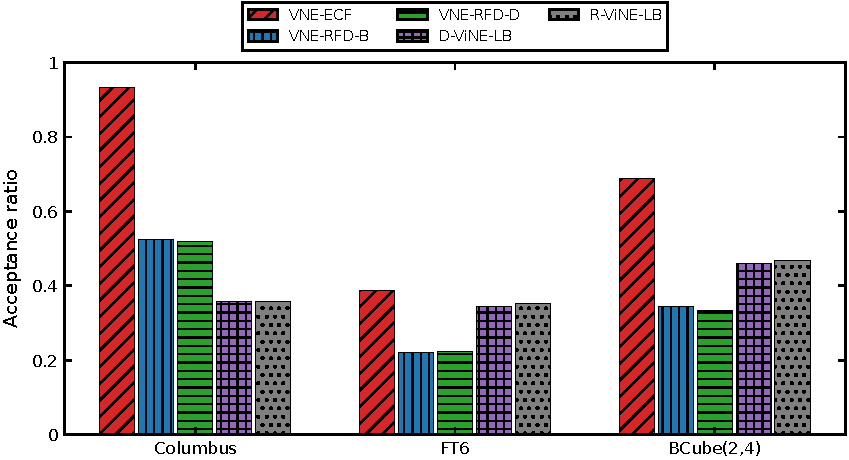
\includegraphics[width=\columnwidth]{figures/fig2_fix_rate_acceptance_ratio.pdf}
    \caption{VNR acceptance ratio.}
    \label{fig:acceptance}
\end{figure}
% Acceptance ratio (arrival rate 40)
%  	VNE-ECF	VNE-RFD-B	VNE-RFD-D	D-ViNE	R-ViNE
% Columbus	0.932193	0.525403	0.519489	0.358104	0.358202
% FT6	0.388311	0.221406	0.222786	0.344010	0.351254
% BCube(2,4)	0.688464	0.343912	0.334056	0.460898	0.467353

\subsubsection{Acceptance Ratio}

Fig.~\ref{fig:acceptance} shows the VNR acceptance ratio under an arrival rate of 40 VNRs per
1{,}000 time units. \ecfvne{} achieves the highest acceptance ratio on all three substrate
networks. On Columbus, \ecfvne{} accepts 93.2\% of the arriving VNRs, compared with 52.5\% and
51.9\% for VNE-RFD-B and VNE-RFD-D and 35.8\% for both D-ViNE and R-ViNE; that is, the acceptance
ratio is improved by a factor of about 1.8 over the fragmentation-based baselines and about 2.6
over the load-balancing baselines. On BCube$(2,4)$, \ecfvne{} accepts 68.8\% of the VNRs, whereas
the best baseline, R-ViNE, accepts 46.7\%, and the RFD-based algorithms accept only about 34\%. On
FT6, all algorithms attain comparatively low acceptance ratios, and \ecfvne{} achieves 38.8\%
against 35.1\% for R-ViNE and about 22\% for the RFD-based algorithms.

Two observations follow from these results. First, the relative ordering of the two baseline
groups reverses between the ISP network and the DCNs. On Columbus, the RFD-based algorithms clearly
outperform D-ViNE and R-ViNE, which is consistent with the premise that fragmentation awareness is
beneficial on heterogeneous topologies. On FT6 and BCube$(2,4)$, however, VNE-RFD-B and VNE-RFD-D
fall well below the load-balancing baselines, accepting only about 64\% and 75\% as many VNRs as
D-ViNE, respectively. We attribute this degradation to the way RFD aggregates the residual
resources of a hop-bounded neighborhood. The link RFD weights each adjacent link by the residual
CPU ratio of the shared node, so every link incident to a zero-CPU switch is assigned the maximum
fragmentation degree irrespective of its residual bandwidth, and the node RFD of a host averages
over a neighborhood that consists mostly of such switches. On a regular topology with uniform
link capacities, the resulting values are nearly identical across hosts and provide little
guidance for node selection. In contrast, \ecfvne{} preserves its advantage on the DCNs
because the external connectivity of a host is evaluated directly through the residual bandwidth
of its attached links, which is exactly the resource that determines whether the host can still
support virtual nodes with incident virtual links. The proposed metric therefore remains
discriminative even when CPU capacities are uniform and the topology is symmetric.

Second, the magnitude of the gain depends on the structural bottleneck of the substrate. On FT6,
each host is attached to the fabric through a single link with a capacity of 100, so the aggregate
bandwidth of all virtual links incident to a virtual node must traverse that single link. Since a
virtual link demand can be as large as 50, this access link constrains the attainable acceptance
ratio of every algorithm, which explains the uniformly low values on FT6 and the smaller relative
improvement of \ecfvne{}. BCube$(2,4)$ provides each host with multiple attachment links, which
relaxes this bottleneck; accordingly, all algorithms achieve higher acceptance ratios and the
benefit of avoiding fragmentation of the host-side bandwidth becomes more pronounced, resulting in
a gain of about 22 percentage points over the best baseline.

\begin{figure}[!t]
    \centering
    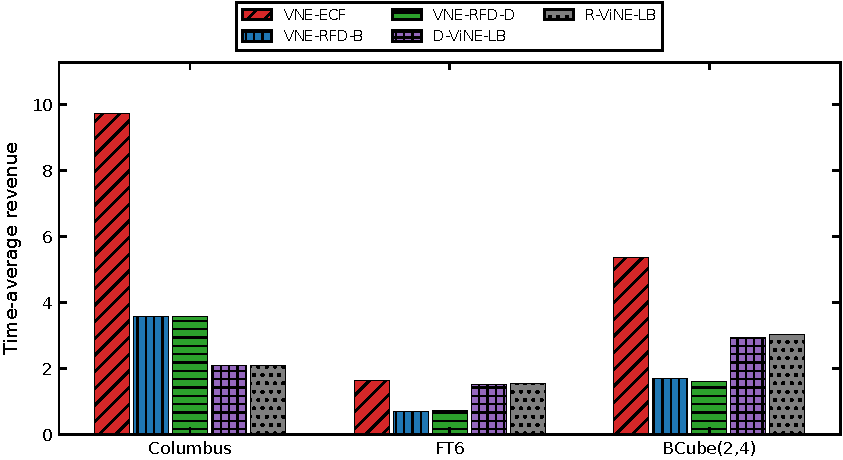
\includegraphics[width=\columnwidth]{figures/fig3_fix_rate_average_revenue.pdf}
    \caption{Time average of generated revenue.}
    \label{fig:revenue}
\end{figure}
% Time-average revenue (arrival rate 40)
%  	VNE-ECF	VNE-RFD-B	VNE-RFD-D	D-ViNE	R-ViNE
% Columbus	9.709791	3.589142	3.572573	2.105087	2.095923
% FT6	1.632458	0.695184	0.717869	1.502564	1.546385
% BCube(2,4)	5.348123	1.685764	1.607970	2.954614	3.038214

\begin{figure}[!t]
    \centering
    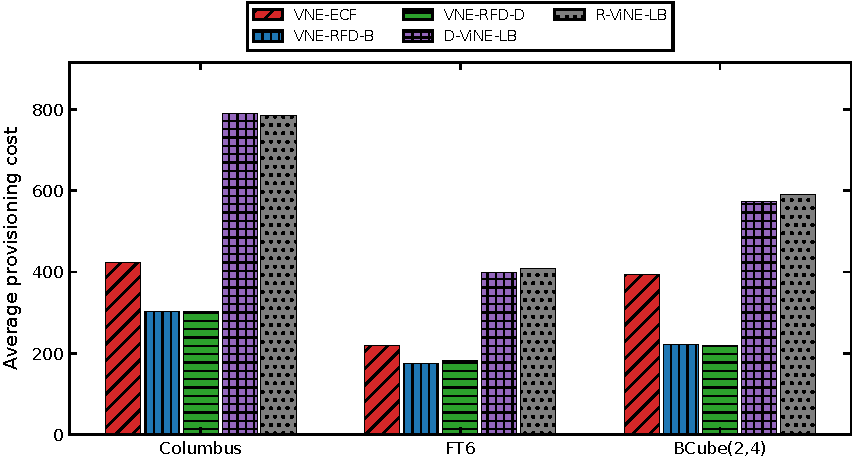
\includegraphics[width=\columnwidth]{figures/fig4_fix_rate_average_cost.pdf}
    \caption{Average embedding cost per accepted VNR.}
    \label{fig:cost}
\end{figure}
% Average provisioning cost (arrival rate 40)
%  	VNE-ECF	VNE-RFD-B	VNE-RFD-D	D-ViNE	R-ViNE
% Columbus	424.002607	302.008206	303.288561	788.874081	785.084744
% FT6	219.578423	175.675998	182.553828	398.586629	408.092600
% BCube(2,4)	392.660787	222.799521	219.380631	573.585859	589.713464

\subsubsection{Revenue and Embedding Cost}

Fig.~\ref{fig:revenue} presents the time-average revenue. The revenue results amplify the
acceptance results because \ecfvne{} not only accepts more VNRs but also sustains a larger number
of concurrently embedded VNRs in the substrate. On Columbus, \ecfvne{} generates about 2.7 times the
revenue of the RFD-based algorithms and about 4.6 times that of the ViNE algorithms. On
BCube$(2,4)$, the corresponding factors are about 3.2--3.3 and 1.8, and on FT6 they are about 2.3 and
1.06--1.09. The comparatively small revenue margin over R-ViNE on FT6 is again a consequence of
the access-link bottleneck discussed above, which limits how much additional demand any algorithm
can accommodate.

Fig.~\ref{fig:cost} shows the average embedding cost per accepted VNR. Here the RFD-based
algorithms attain the lowest cost on all networks, \ecfvne{} incurs a moderately higher cost, and
D-ViNE and R-ViNE incur the highest cost. The cost of \ecfvne{} is 1.25 to 1.76 times that of
VNE-RFD-B but only 54\% to 68\% of that of D-ViNE. The higher cost relative to the RFD-based
algorithms should be interpreted together with the acceptance ratio: \ecfvne{} accepts VNRs that
the RFD-based algorithms reject, and these additional VNRs are embedded in a substrate whose
residual capacity is more heavily utilized, so their virtual links are routed over somewhat longer
paths. Moreover, the objective of \ecfvne{} deliberately trades a small increase in the present
embedding cost for lower induced fragmentation whenever a slightly longer path leaves the remaining
resources better connected. Despite this, the revenue generated per unit of embedding cost is the
highest for \ecfvne{} on every network, indicating that the additional cost is more than
compensated by the increase in accepted demand. The ViNE algorithms, by contrast, spread traffic
over the substrate for load balancing and therefore consume substantially more bandwidth per
accepted VNR, which manifests as both a higher cost and a lower acceptance ratio.

\begin{figure*}[!t]
    \centering
    \begin{subfigure}[b]{0.48\textwidth}
        \centering
        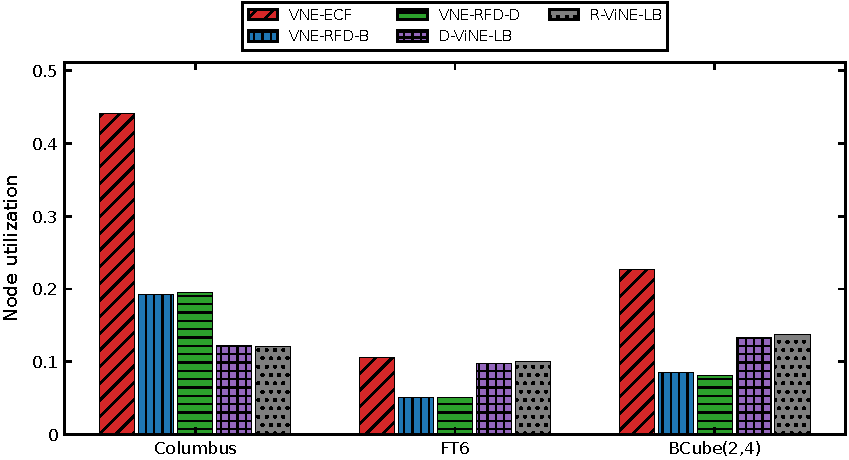
\includegraphics[width=\textwidth]{figures/fig5_a_fix_rate_avg_node_utilization.pdf}
        \caption{Average node utilization.}
        \label{fig:node_util}
    \end{subfigure}
    \hfill
    \begin{subfigure}[b]{0.48\textwidth}
        \centering
        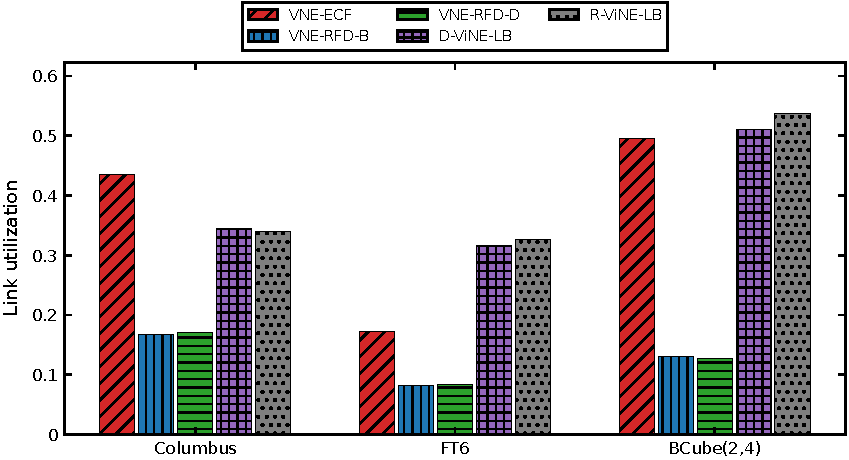
\includegraphics[width=\textwidth]{figures/fig5_b_fix_rate_avg_link_utilization.pdf}
        \caption{Average link utilization.}
        \label{fig:link_util}
    \end{subfigure}
    \caption{Average substrate resource utilization.}
    \label{fig:util}
\end{figure*}
% Node utilization (arrival rate 40)
%  	VNE-ECF	VNE-RFD-B	VNE-RFD-D	D-ViNE	R-ViNE
% Columbus	0.440480	0.192645	0.194784	0.122629	0.121004
% FT6	0.105337	0.050802	0.051106	0.098186	0.100411
% BCube(2,4)	0.227092	0.084828	0.081123	0.133850	0.137675
% Link utilization (arrival rate 40)
%  	VNE-ECF	VNE-RFD-B	VNE-RFD-D	D-ViNE	R-ViNE
% Columbus	0.434512	0.167537	0.171434	0.344444	0.339634
% FT6	0.172929	0.082441	0.084033	0.316808	0.326932
% BCube(2,4)	0.494536	0.130920	0.126637	0.510461	0.536424

\subsubsection{Resource Utilization}

Fig.~\ref{fig:util} shows the average node and link utilization. \ecfvne{} achieves the highest
node utilization on all networks, about 2.1 to 2.7 times that of the RFD-based algorithms and 1.1
to 3.6 times that of the ViNE algorithms. Since node utilization is proportional to the CPU demand
of the VNRs that are simultaneously embedded, this result confirms that the higher acceptance ratio
of \ecfvne{} translates into a correspondingly larger amount of admitted demand rather than into
the admission of small requests only.

Link utilization reveals a more subtle difference between the two baseline groups. On Columbus,
\ecfvne{} also attains the highest link utilization. On FT6 and BCube$(2,4)$, however, D-ViNE and
R-ViNE reach link utilizations comparable to or higher than that of \ecfvne{} even though they
accept fewer VNRs and admit less CPU demand. The ratio of link utilization to node utilization is
about 3.2 to 3.9 for the ViNE algorithms but only 1.6 to 2.2 for \ecfvne{}, which means that the
ViNE algorithms consume roughly twice as much bandwidth per unit of admitted CPU demand. This is
the utilization-side counterpart of their high embedding cost: load balancing distributes the
flows of a VNR over longer paths, occupying bandwidth on many links without a corresponding
increase in accepted requests. The RFD-based algorithms exhibit the lowest utilization of both
resources, which reflects their conservative admission rather than efficient use of the substrate.
\ecfvne{} thus converts substrate capacity into accepted VNRs most efficiently, keeping the
consumption of bandwidth in proportion to the admitted demand while leaving the residual resources
in a combinable state.

\subsubsection{Running Time}

% 런타임 그림은 일단 보류
% \begin{figure}[!t]
%     \centering
%     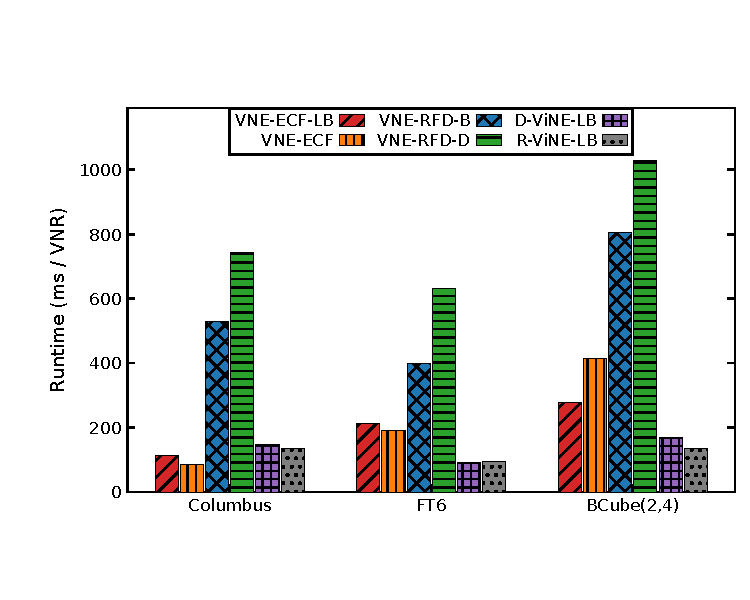
\includegraphics[width=\columnwidth]{figures/fig6_fix_rate_runtime_ms_per_vnr.pdf}
%     \caption{Average runtime per VNR.}
%     \label{fig:runtime}
% \end{figure}
% Runtime (ms / VNR, arrival rate 40)
%  	VNE-ECF	VNE-RFD-B	VNE-RFD-D	D-ViNE	R-ViNE
% Columbus	1.560100	605.417379	771.508487	134.769023	125.768475
% FT6	1.474476	409.887678	631.778218	96.645303	84.955590
% BCube(2,4)	1.905753	853.542868	1217.085351	138.652401	117.097019

The average running time per VNR of \ecfvne{} is between 1.5 and 1.9\,ms on all three networks. The
ViNE algorithms require 85 to 139\,ms per VNR because they solve a linear programming relaxation
for every request, and the RFD-based algorithms require 410 to 1{,}217\,ms per VNR owing to their
backtracking search over $K$ candidate paths and hop-bounded neighborhood evaluation. The low
running time of \ecfvne{} is consistent with the complexity bound~\eqref{eq:complexity}: the induced fragmentation cost is evaluated locally from the
residual bandwidth of adjacent links, so the additional cost of fragmentation awareness over a
plain greedy embedding is small.

\subsection{Results Under Increasing Arrival Rates}

\begin{figure*}[!t]
    \centering
    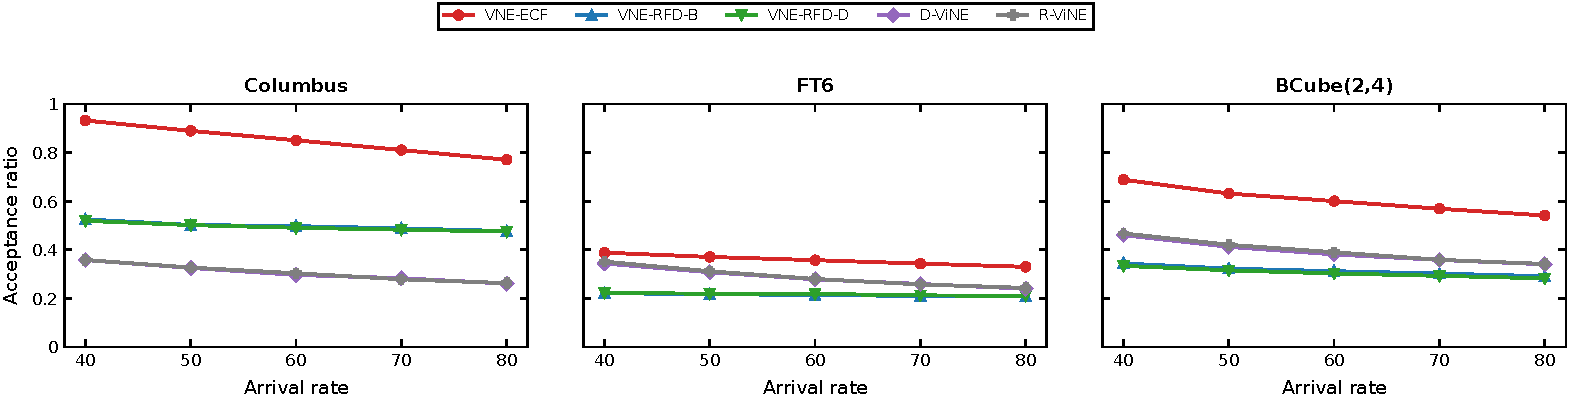
\includegraphics[width=\textwidth]{figures/fig7_acceptance_arrival_rate.pdf}
    \caption{VNR acceptance ratio under increasing arrival rates for the Columbus, FT6, and BCube(2,4) substrate networks.}
    \label{fig:acceptance_arrival_rate}
\end{figure*}
% Acceptance values — Columbus
%  	VNE-ECF	VNE-RFD-B	VNE-RFD-D	D-ViNE	R-ViNE
% 40	0.932193	0.525403	0.519489	0.358104	0.358202
% 50	0.889590	0.502031	0.501755	0.325589	0.326890
% 60	0.850651	0.497380	0.490789	0.296886	0.303411
% 70	0.810582	0.488227	0.482894	0.283064	0.278723
% 80	0.770541	0.476972	0.475211	0.260807	0.262816
% Acceptance values — FT6
%  	VNE-ECF	VNE-RFD-B	VNE-RFD-D	D-ViNE	R-ViNE
% 40	0.388311	0.221406	0.222786	0.344010	0.351254
% 50	0.370715	0.217940	0.219242	0.307956	0.311704
% 60	0.357423	0.213742	0.218718	0.278728	0.279980
% 70	0.343348	0.210525	0.212511	0.259319	0.257674
% 80	0.329903	0.207733	0.210511	0.239875	0.243050
% Acceptance values — BCube(2,4)
%  	VNE-ECF	VNE-RFD-B	VNE-RFD-D	D-ViNE	R-ViNE
% 40	0.688464	0.343912	0.334056	0.460898	0.467353
% 50	0.631612	0.322551	0.315609	0.412410	0.420615
% 60	0.600428	0.312078	0.302719	0.381117	0.390015
% 70	0.569050	0.302184	0.292965	0.358496	0.358922
% 80	0.541157	0.291188	0.282582	0.340344	0.341609

To examine the robustness of the results with respect to the offered load, we vary the VNR arrival
rate from 40 to 80 arrivals per 1{,}000 time units while keeping all other settings fixed.
Fig.~\ref{fig:acceptance_arrival_rate} shows the resulting acceptance ratios. \ecfvne{} retains the
highest acceptance ratio at every arrival rate on every substrate network; no crossover with any
baseline is observed within the tested range.

The acceptance ratio of every algorithm decreases as the arrival rate increases, but the rate of
decrease differs markedly across algorithm groups. The load-balancing baselines degrade most
rapidly, losing 26\% to 31\% of their acceptance ratio between the lowest and highest arrival
rates on all three networks. The RFD-based algorithms degrade the least, by 6\% to 15\%, but from
an already low level; their acceptance is limited primarily by their conservative embedding
decisions rather than by the offered load, so additional load has a comparatively small effect.
\ecfvne{} lies in between, with a relative decrease of 15\% to 21\%. Because \ecfvne{} operates
much closer to the capacity of the substrate, it is naturally more exposed to the increased
contention, yet its acceptance ratio at the highest arrival rate remains above the acceptance
ratio of every baseline at the lowest arrival rate on Columbus and BCube$(2,4)$.

The evolution of the margin over the strongest baseline is also informative. On Columbus, the
absolute gap over VNE-RFD-B narrows from about 41 to 29 percentage points as the load increases,
while the acceptance ratio of \ecfvne{} remains 1.6 times that of VNE-RFD-B at the highest rate. On
BCube$(2,4)$, the gap over the ViNE algorithms is essentially constant at about 20 to 22 percentage
points, and the ratio increases from 1.47 to 1.58. On FT6, the margin widens with load: the gap
over R-ViNE grows from about 4 to 9 percentage points and the ratio from 1.11 to 1.36, because the
ViNE algorithms lose acceptance quickly while \ecfvne{} degrades gracefully. This indicates that
the advantage of preserving the combinability of residual resources becomes more pronounced as the
substrate becomes more congested, since under heavier load a fragmented residual state is
increasingly likely to cause the rejection of otherwise feasible requests. Overall, the results
show that the improvement of \ecfvne{} is not specific to a particular operating point but
persists, and in the DCNs even strengthens, as the offered load increases.

\section{Conclusion}
\label{sec:conclusion}

This paper addressed the problem of resource fragmentation in online VNE, in which residual
substrate resources remain available in aggregate but become difficult to combine into the node
and link resources required by future requests. We proposed the External-Connectivity-based
Fragmentation (\ecf{}) metric, which expresses the usability of a residual resource as the product
of its residual amount and the deficiency of its normalized external connectivity. External
connectivity is defined through the residual capacity of the boundary cut between a resource region
and its exterior, which gives it a direct interpretation and guarantees that it is monotone under
embedding without any hop-count or neighborhood parameter. The metric is specialized for substrate
nodes and links according to the distinct resource combinations required by node embedding and
virtual-link routing. We further decomposed the change in fragmentation caused by an embedding into
direct resource consumption and the degradation of the connectivity of the remaining resources, and
defined the latter as the induced fragmentation cost, which is non-negative by construction. Based
on this cost, we formulated the online embedding problem and proposed \ecfvne{}, a greedy algorithm
that embeds each virtual node and its pending virtual links so as to minimize the induced
fragmentation cost relative to the pre-request substrate state.

Simulation results on an ISP topology and on FatTree and BCube data center topologies showed that
\ecfvne{} achieves the highest acceptance ratio, revenue, and node utilization among the compared
algorithms on every topology and at every tested arrival rate, under an algorithmic structure
comparable to that of the RFD-based baselines but without backtracking. In particular, whereas the existing
fragmentation-aware baselines outperform the load-balancing baselines on the heterogeneous ISP
topology but fall below them on the regular data center topologies, \ecfvne{} retains its advantage
in both environments, because the external connectivity of a host is evaluated directly from the
residual bandwidth of its attached links. The margin of \ecfvne{} over the strongest baseline
persists as the arrival rate increases and widens on the FatTree topology, indicating that
preserving the combinability of residual resources becomes more valuable under heavier load. The
additional embedding cost incurred relative to the fragmentation-aware baselines is more than
compensated by the increase in accepted demand, and the algorithm runs in a few milliseconds per
request.

Several directions remain for future work. The weighting factors of the induced fragmentation cost
were fixed in this study; adapting them to the observed CPU and bandwidth scales or to the current
load of the substrate may further improve performance. The external connectivity of a single node
or link could be extended to larger resource regions in order to capture fragmentation at the
scale of multi-node subgraphs. Finally, combining the induced fragmentation cost with path
splitting or with request reordering and admission control, and evaluating the metric in
substrates with additional resource types such as storage or heterogeneous accelerators, are
promising extensions of the proposed framework.

% \nocite{*}
\bibliographystyle{IEEEtran}
\bibliography{references}

\newpage

\begin{IEEEbiography}[{
\includegraphics[width=1in,height=1.25in,clip,keepaspectratio]{authors/jae_hong_jung_photo.jpg}}]{Jae-Hong Jung} received his B.S. degree in Computer Science and Engineering from Inha University, Incheon, South Korea, in 2025. He is currently pursuing an M.S. degree in Computer Science and Engineering in the Department of Electrical and Computer Engineering at Inha University. He is conducting research on Virtual Network Embedding (VNE) in the Network Laboratory. His research interests include Software-Defined Networking (SDN), Network Function Virtualization (NFV), and network virtualization.
\end{IEEEbiography}

\begin{IEEEbiography}[{
\includegraphics[width=1in,height=1.25in,clip,keepaspectratio]{authors/bon_seung_ku.jpg}}]{Bon-Seung Ku} received his B.S. degree in Computer Science and Engineering from Inha University, Incheon, South Korea, in 2025. He is currently pursuing an M.S. degree in Computer Science and Engineering in the Department of Electrical and Computer Engineering at Inha University. He is conducting research on Virtual Network Embedding (VNE) in the Network Laboratory. His research interests include Software-Defined Networking (SDN), Network Function Virtualization (NFV), and network virtualization.
\end{IEEEbiography}

\begin{IEEEbiography}[{
\includegraphics[width=1in,height=1.25in,clip,keepaspectratio]{authors/gu_in_kwon_photo.jpg}}]{Gu-In Kwon} received his M.A. degree in Computer Science from Queens College, City University of New York, in 1998, and his Ph.D. degree in Computer Science from Boston University, Boston, MA, USA, in January 2005. He is currently a Professor in the Department of Computer Science and Engineering at Inha University, Incheon, South Korea. His research interests include Network Function Virtualization (NFV) and cloud computing.
\end{IEEEbiography}

\EOD
\end{document}
